\documentclass[11pt]{article}

\usepackage[bindingoffset=0cm,centering,includeheadfoot,margin=2cm]{geometry}
\usepackage{float}
\usepackage{parskip}
\usepackage{xspace}
\usepackage{color}
\usepackage{textcomp}
\usepackage{flafter}
%\usepackage{longtable}
\usepackage{amssymb}
\usepackage{def+cmd}
\usepackage{graphicx}
\usepackage{subcaption}
%\usepackage{verbatim}
%\usepackage{stackrel}
%\usepackage{fancyvrb}
%\usepackage{bm}
%\usepackage{algorithm}
%\usepackage{algorithmic}
%\newcommand{\theHalgorithm}{\arabic{algorithm}}
% CLRS uses a right-facing black triangle for comments:
%\newcommand*\alcom{\STATE\ensuremath{\blacktriangleright} }

\usepackage[printwatermark]{xwatermark}
\newwatermark[allpages,color=red!15,angle=60,scale=6,xpos=-15mm,ypos=15mm]{DRAFT}
%\draftfalse
%\usepackage{editorial}

\usepackage[american]{circuitikz}

\newcommand*\mytitle{Electricity Primer for Renewable Energy Technologies}
\newcommand*\mysubtitle{ENERGY-293C, Fall 2015}

\newcommand*\doctitle{{\mytitle} \\ {\Large{\mysubtitle}}}
\newcommand*\docauthor{Emmet Caulfield}

\usepackage{ifpdf}
\ifpdf
  \usepackage{epstopdf}
  \DeclareGraphicsExtensions{.pdf,.eps,.png,.jpg}
\fi


\graphicspath{{figures/}{figures/raster/}}

\usepackage{booktabs}
\usepackage{dcolumn}
\newcolumntype{d}[1]{D{.}{.}{#1}}
\newcommand*\dch[1]{\multicolumn{1}{c}{#1}}

\usepackage{hyperref}
\hypersetup{
  plainpages=true,
  colorlinks=true,
  linkcolor=blue,
  citecolor=black,
  pagecolor=black,
  urlcolor=blue,
  pdftitle=\doctitle,
  pdfauthor=\docauthor,
  pdfsubject={},
  pdfkeywords={},
  pdfcreator={$ $Id: paper.tex 58 2013-11-16 00:29:54Z emmet $ $},
  pdfproducer={pdfTeX using libpoppler 3.141592-1.40.3-2.2 (Web2C 7.5.6)}
}

%\usepackage[acronym]{glossaries} % Must be after hyperref

%\usepackage{listings}
%\lstset{
%  basicstyle=\tiny\ttfamily,
%  keywordstyle=\bfseries,
%  showstringspaces=false,
%  frame=tb
%}

% Without these, LaTeX tends to move floats toward the end of
% the document:
\renewcommand{\topfraction}{0.9}	% 90% of page top can be a float
\renewcommand{\bottomfraction}{0.9}	% 90% of page bottom can be a float
\renewcommand{\textfraction}{0.1}	% only 10% of page must to be text

% It can be handy to decide how wide we want figures to be on
% a document-wide basis.
\newlength\onewide
\setlength\onewide{0.9\textwidth}
\newlength\onenarrow
\setlength\onenarrow{0.6\textwidth}
\newlength\twowide
\setlength\twowide{0.4\textwidth}

% As big as a graph can be to fit two high on a page:
\newlength\onehigh
\setlength\onehigh{0.97\textheight}
\newlength\twohigh
\setlength\twohigh{0.425\textheight}


% Whether we want separate sections or not:
\newif\ifclearpagesection
\newif\ifclearpageappendix
\clearpageappendixtrue
\newif\ifclearpageglossary
\clearpageglossaryfalse
\newif\ifclearpagebibliography
\clearpagebibliographytrue

\newcommand{\fixme}[1]{{\color{red}{\bf FIXME:} #1}}
\newcommand\citeme{{\color{red}{\bf??}}}

%% Results/setup values from R:
\input{figures/results.tex}


\author{\docauthor}
\title{\doctitle}
%\date{September 23, 2006}

\begin{document}
\maketitle

\section{Assumptions}

We assume that everybody is broadly familiar with the most basic ideas
of electricity, in particular:

That \term{current} --- measured in amperes\footnote{Although named
  for Amp\`ere, the SI unit does not bear an accent.}, symbol~\unit{A}
--- is the flow rate of electric \term{charge} --- measured in
coulombs, symbol~\unit{C}.
\[
1~\unit{A} = 1~\unit{C}{s}
\]

That there are two kinds of charge, \emph{positive} and
\emph{negative}, that like charges repel each other and unlike charges
attract each other according to \term{Coulomb's Law}: an
inverse-square force law:
\[
\vec{F}_\mathrm{C} = \frac{Q_1 Q_2}{4\pi\epsilon\abs{\vec{r}_{12}}^2}\hat{r}_{12}
\]

That the predominant --- for our purposes exclusive --- charge-carrier
is the negatively-charged \term{electron}, which carries a charge of
$\approx-1.6\times 10^{-19}~\unit{C}$, the magnitude of which is called the
\term{elementary charge} and denoted\footnote{To avoid confusion with
  Euler's number, $\mathrm{e}$, we will use $q$.} $e$ or $q$.

That, for historical reasons, \term{conventional current} is
conceptualized as the flow of \emph{positive} charge but, in reality,
negatively charged electrons are flowing in the opposite direction.

That this is arbitrary and immaterial to circuit analysis.

That \term{electric potential difference}, or just \term{potential
  difference}, colloquially ``\term{voltage}'' is a measure of the
difference in potential energy (in joules) per unit charge (in
coulombs) between two points; the unit, the \term{volt},
symbol~\unit{V}, is a joule-per-coulomb.
\[
1~\unit{V} = 1~\unit{J}{C}
\]

That electric fields and currents obey the principle of linear
superposition.

That different materials impede the flow of electrons to different
degrees. The property that quantifies this effect between two points
on an object is \term{resistance}, measured in ohms, symbol~\unit{\Omega}.

That the bulk material property that quantifies this effect is
\emph{resistivity}, measured in ohm-meters, symbol~\unit{\Omega\cdot m}.

That the relationship between the potential difference between two
points, the resistance between those points, and the current that
flows from one point to the other is given by \term{Ohm's Law}:
\begin{equation}
\label{eqn:vir}
V = I\times R
\end{equation}

\begin{figure}[ht]
  \centering
  \begin{circuitikz}
    \draw (0,0) to [short, i=$I$] (2,0);
    \draw (2,0) to [R=$R$, v=$V$] (4,0);
    \draw (4,0) to [short] (6,0);
  \end{circuitikz}
  \caption{Resistor Labeled with Current and Voltage}
  \label{fig:ohmslaw}
\end{figure}


That the reciprocal of resistance is \term{conductance} and has units
of siemens, symbol \unit{S}.

That the reciprocal of resistivity is \term{conductivity} and has
units of siemens per meter, symbol \unit{S}{m}.

That (DC) electric power consumed by a resistance is the product of
potential difference and current:
\[
P = I\times V = I^2\times R = \frac{V^2}{R}
\]

%\begin{abstract}
This document is an electricity primer that begins with first principles.
\end{abstract}

\section{Electricity}

The electromagnetic interaction is one of the four fundamental forces
of nature.

Historically, electricity and magnetism were conceptualized as being
different but connected, which is reflected in classical classroom
treatments that treat electricity and magnetism as two different
phenomena that interact. In fact, magnetism is a relativistic
consequence of the movement of electric charge.

For our purposes the classical phenomenological description is more
than adequate.

\subsection{Electrostatics}

\subsubsection{Charge Carriers and Continuity}

In this description, charge is treated as a continuously variable
scalar quantity with two types: ``positive'' and ``negative''. Like
charges repel each other and unlike charges attract each other. The
S.I. unit of charge is the \emph{coulomb}\footnote{S.I. units are
  treated as common nouns and are \emph{not} capitalized other than at
  the beginning of a sentence.}, symbol \emph{C}\footnote{The symbols
  for S.I. units named after persons, and \emph{only} those S.I units,
  are \emph{always} capitalized.}.

In the best current theory, charge is ultimately carried by a number
of \term{elementary particles}\footnote{Specifically electrons, muons,
  tau leptons, quarks, and their respective antiparticles.} but for
almost all practical purposes in electrical and electronic
engineering, the only real charge-carrier is the negatively charged
electron. There are a few circumstances where positive charge occurs
in practice --- as ions in plasma and in solutions in electrochemistry
--- but outside of a handful of exceptions, when we talk about a
positive charge in electrical and/or electronic engineering, it's a
convenient fiction or an abstraction: what's really going on is all
about electrons.

An electron carries a charge of $\approx
-1.6\times10^{-19}\unit{C}$. Compared to the amounts of charge we deal
with in practice, this is so minuscule that there's no problem with
the assumption of continuity.

\subsubsection{The Coulomb Force}

Charges exert a force on each other, sometimes called the
\term{Coulomb force} to distinguish it from other forces. 

The force, in newtons (\unit N), experienced by a charge, $Q_1$, at a
fixed position, $\vec{r}$, relative to another charge, $Q_0$, at the
origin, is given by an inverse-square law much like Newton's Law of
Gravitation, called \term{Coulomb's Law}:

\begin{equation}
\label{eqn:coulombs}
F(\vec{r}) = \frac{1}{4\pi\epsilon}\frac{Q_0 Q_1}{|\vec{r}\,|^2} \hat{r} \qquad\bunit{N}{C}
\end{equation}

Where $\hat{r}$ is the unit-vector from the origin to $Q_1$ and
$\epsilon$ is the \term{permittivity} of the ``universe'' where the
two charges sit. As you might expect, $Q_0$ experiences the same
force, but in the opposite direction, $-\hat{r}$.

Permittivity can be thought of as a property of a material that says
how effectively it blocks the electric force: the higher the
permittivity, the lower the Coulomb force experienced by the two
charges. We won't have much need for discussing permittivity, but just
to give you an idea of its magnitude, the \term{permittivity of free
  space} or \term{vacuum permittivity} is about 8.85\unit{F}{m}
(farads\footnote{more about farads later} per meter).

Note that, in general, permittivity is a tensor quantity, since many
materials have different permittivities in different directions: think
of materials like mica or graphite.

\subsubsection{Linear Superposition}

Electrical charge obeys the principle of linear superposition. That is
to say that the total force experienced by a charge, $Q_2$, due to two
other charges, $Q_1$ and $Q_0$, is just the vector sum of the forces
that $Q_2$ would feel due to each of the other charges considered
individually.

\subsubsection{Electric Field}

The \emph{electric field} due to some configuration of charges is just
the force per unit charge that would be experienced by a positive
charge due to that configuration of charges according to Coulomb's
Law. Not surprisingly, the E-field has units of newtons (force) per
coulomb (charge) and is a vector quantity.

The E-field (in \unit{N}{C}) experienced by a charge, $Q_1$, at a
position $\vec{r}$ relative to another charge, $Q_0$, at the origin
follows directly from Coulomb's Law (above):

\begin{equation}
\label{eqn:efield}
E(\vec{r}) = \frac{1}{4\pi\epsilon}\frac{Q_0}{|\vec{r}\,|^2} \hat{r} = \frac{F(\vec{r})}{Q_1} \qquad\bunit{N}{C}
\end{equation}

You can probably imagine that if you placed a positive charge on one
of the black \term{field lines} of Figure~\ref{fig:positive}, it
would be accelerated away from the charge shown in the center along
the same field line. The further away it gets, the weaker the
accelerating force becomes, so while the field lines indicate the
direction a positive charge will move, how close together the field
lines are is an indication of the strength of the field.

\begin{figure}[H]
  \centering
  \begin{subfigure}[b]{\twowide}
    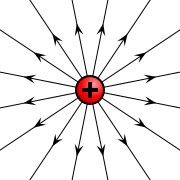
\includegraphics[width=\twowide]{positive}
    \caption{Positive Charge}
    \label{fig:positive}
  \end{subfigure}
  \begin{subfigure}[b]{\twowide}
    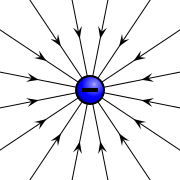
\includegraphics[width=\twowide]{negative}
    \caption{Positive Charge}
    \label{fig:negative}
  \end{subfigure}
  \caption{Electric Field Due to An Isolated Point Charge}
  \label{fig:onecharge}
\end{figure}

Electro\emph{static} fields are conservative\footnote{As we will see,
  things change a little for time-varying electric fields.}. In other
words, if you moved a charge from a point, $a$, to another point, $b$,
in an electrostatic field, the amount of work you would have to do is
independent of the path, $\ell$, taken from $a$ to $b$. Moreover, if
you moved a charge through a closed loop from $a$ back to $a$ again,
you would do no net work, no matter how big or small the loop or how
circuitous its path.

\begin{equation}
\oint_\ell \vec{E}\cdot\dee{\vec{\ell}} = 0
\end{equation}
or
\begin{equation}
\curl{E} = 0
\end{equation}

\subsubsection{Electric Potential}

Mathematically, a conservative vector field is the gradient of some
scalar field:
\begin{equation}
\vec{E} = -\grad\phi \qquad\bunit{N}{C}
\end{equation}
or
\begin{equation}
\phi = -\int \vec{E}\cdot\vec{\dee\ell} \qquad\bunit{N\cdot m}{C}
\end{equation}

The unit of newton-meters, or joules\footnote{Recall that the joule is
  \emph{defined} as the work done when an object is moved one meter
  against a force of one newton.}, per coulomb is called the
\term{volt}:
\begin{equation}
V = \unit{N\cdot m}{C} = \unit{J}{C}
\end{equation}

Figure~\ref{fig:dipole} shows the $\vec{E}$-field and equipotential
contours of an electrostatic dipole. Note that the $\vec{E}$-field
lines are everywhere perpendicular to the isolines of electric
potential.

Conventionally, the units of electric field are given as volts per
meter, which is equivalent to the earlier units of newtons per
coulomb:

\begin{equation}
\unit{V}{m} = \frac{\unit{N\cdot m}{C}}{\unit{m}} = \unit{N\cdot m}{C}\cdot\unit{1}{m} = \unit{N}{C}
\end{equation}
%\int_a^b \vec{E}\cdot\dee{\vec{\ell}} = \phi|_b - \left.\vec{E}\right|_a

\begin{figure}[ht]
  \centering
  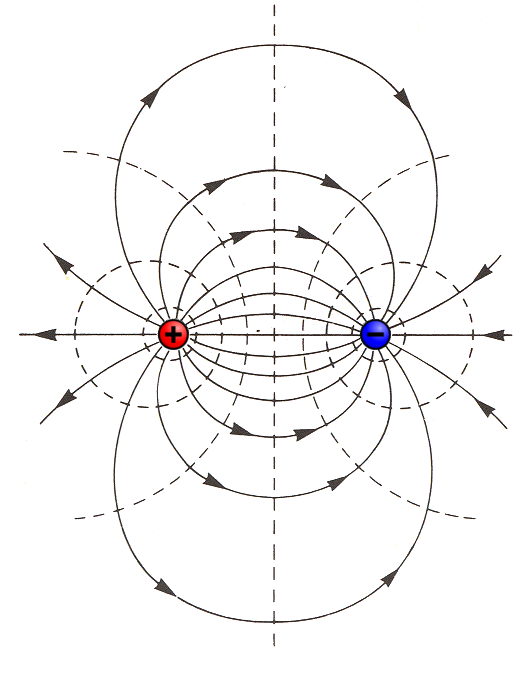
\includegraphics[width=\onenarrow]{potential-dipole}
  \caption{Field Lines and Equipotential Contours of a Dipole}
  \label{fig:dipole}
\end{figure}

So the electric potential at a point, $p$, in an electric field is the
work done (or yielded) by moving a point charge, $Q$, from where the
E-field is zero (infinitely far away from any charges) to that point
per coulomb of $Q$'s charge.

\subsubsection{Electric Potential Difference}

As for other scalar potential fields, we're generally more interested
in differences in potential than in absolute potentials. The electric
potential difference, colloquially called \term{voltage}, is
(unsurprisingly) just the difference in electric potential between two
points.

So, {\bf ``voltage'' is a measure of electric potential energy,
  measured in units of energy per unit charge or joules per
  coulomb}. This is analgous to gravitational potential in joules per
  unit mass, or pressure in joules per unit volume.

Consider, for example, the familiar equation for gravitiational
potential energy, $E_\mathrm{GP} = mgh$. This can be viewed as the
gravitational potential difference of an object of mass, $m$, on the
ground and the same object raised to a height, $h$. The analog of
``voltage'', then, would be the $gh$ product, which should have units
of joules per kilogram (by analogy with joules per coulomb), and so it
does:

\begin{equation}
g\bunit{m}{s^2}\cdot h\bunit{m} = gh\left[\unit{m^2}{s^2}\cdot\unit{kg}{kg}\right] = gh\left[\unit{kg\cdot m^2}{s^2}\cdot\unit{1}{kg}\right] = gh\bunit{J}{kg}
\end{equation}


\subsubsection{Charge Distributions}

Suppose you did that old trick where you rub your hair with a balloon,
then hold it a few inches away from your head so it lifts your hair
up\footnote{Assuming that your hair is fine enough, long enoug, and
  the relative humidity is low enough}.

On the head side of the balloon, there is a surface distribution of
negative charge. Your hairs, on the other hand, have a net positive
charge. The unlike charges attract, and your hair is lifted toward the
balloon. The like charges on the hairs repel each other, and the hairs
spread out.

The point is that, in classic electromagnetic theory, you can have
arbitrary surface and volume distributions of charge, not just point
charges.


\subsubsection{Current}

The macroscopic net movement of charge is called \term{current}.

In a copper wire, electrons are constantly whizzing around the nuclei
of the copper atoms, but we don't call this a current: we're only
interested in \emph{net} movement of charge at, at least, a
super-atomic level. In semiconductors, admittedly, the scales where we
talk about current can be very small, but we're still concerned with
net movement.

Not surprisingly, current is measured in units of charge per unit
time, or coulombs per second. A coulomb per second is called an
\term{amp\`ere}.

Strictly speaking, it's the other way around: the amp\`ere is an SI
fundamental unit and the coulomb, or amp\`ere-second, is the derived
unit.

\subsubsection{Ohm's Law}

So what, one might reasonably ask, is the relationship between
potential difference and current in a medium that permits charge to
move?

Intuitively, one would expect that the greater the potential
difference, the greater the amount of current that will flow.

But, as you might expect, it's also dependent on the medium: some
media impede the flow of charge-carriers --- electrons --- more than
others. As a bulk material property, this is called
\emph{resistivity}. As a property of an object, such as a circuit
element or a cable, it is called \emph{resistance}.

If an object has a potential difference of $V_\mathrm{R}$ volts across
its ends, and that causes a current of $I_\mathrm{R}$ amp\`eres to
flow, then the object's resistance, $R$, is given by:

\begin{equation}
R = \frac{V_\mathrm{R}}{I_\mathrm{R}} \qquad\left[\unit{V}{A}=\unit{\Omega}\right]
\end{equation}

Simple, eh?

The unit of volts per amp\`ere has a special name, the \term{ohm},
symbol \unit{\Omega}.


\section{Electrodynamics}


\subsection{Circuit Diagrams}

Having introduced the zig-zag circuit symbol for a resistor in
Figure~\ref{fig:ohmslaw}, it may be helpful to briefly mention
\term{circuit diagrams} or \term{schematics}, which depict circuit
elements or components and how they are connected to each other.

Section~\ref{sec:circuit-elements}, below, contains a reasonably
comprehensive description of the most common circuit symbols. At this
stage, it's useful to know a little about circuit diagrams in general,
even if we can't discuss some important circuit symbols until after
we've reviewed alternating current concepts in
Section~\ref{sec:alternating-current}.


\subsubsection{Types of Circuit Diagram}

There are really two kinds of circuit diagram, which are somewhat
different, they can describe:

\begin{itemize}
  \item a physical assembly of real-world non-ideal components for assembly/production; and
  \item a theoretical assembly of ideal components for analysis/simulation.
\end{itemize}

The example of Figure~\ref{fig:flashlight} shows a ``production''
schematic for a flashlight: the positive terminal of a 3~\unit{V}
battery is connected via a latching switch to a lamp, the other
terminal of which is connected to the chassis. The battery's negative
terminal is also connected to the chassis, completing the circuit.

Figure~\ref{fig:flashlight} also shows an ``analysis'' schematic for
the same flashlight --- admittedly an outlandish pedagogical
contrivance --- but this time the battery is modeled as a 3~\unit{V}
independent voltage source in series with a resistance, $R_B$,
representing the internal resistance of the battery. The switch is
generic (for analysis purposes, we don't care if it latches or not),
the negative terminal of the battery is connected explicitly to the
lamp, and that node is connected to ground.

\begin{figure}[H]
  \centering
  \begin{subfigure}{\twowide}
    \centering
    \begin{circuitikz}
      \draw (0,0) node[cground] {};
      \draw (0,0) to [battery,v=$3~\unit{V}$] (0,2);
      \draw (0,2) to [lspst] (2,2);
      \draw (2,2) to [lamp] (2,0) node[cground] {};
    \end{circuitikz}
    \caption{Production}
  \end{subfigure}
  \begin{subfigure}{\twowide}
    \centering
    \begin{circuitikz}
      \draw (0,0) node[ground] {};
      \draw (0,0) to [V=$3~\unit{V}$] (0,2);
      \draw (0,2) to [R=$R_\mathrm{B}$] (2,2);
      \draw (2,2) to [spst] (4,2);
      \draw (4,2) to [lamp] (4,0);
      \draw (4,0) to [short] (0,0);
    \end{circuitikz}
    \caption{Analysis}
  \end{subfigure}
  \caption{Production and Analysis Schematics for a Flashlight}
  \label{fig:flashlight}
\end{figure}


\section{Alternating Current}
\label{sec:alternating-current}

When we speak of an \term{alternating current}, \term{AC}, we are
usually referring to a sinusoidally time-varying \emph{voltage}
(potential difference). The nominal domestic AC service voltage, \ruVm at
\ruF, can be described by:
\[
v(t) = \rnVm\sqrt{2}\cos(\rnF\cdot 2\pi t+\phi)\qquad\bunit{V}
\]

\ldots where $t$ is time and $\phi$ is some arbitrary phase shift that
depends on what you define as ``time zero'', $t=0$. If you synchronize
your ``time zero'' to a peak, then $\phi=0$ and the potential
difference varies with time as shown in Figure~\ref{fig:ac}.

\begin{figure}[ht]
  \centering
  \includegraphics[width=\onewide]{ac}
  \caption{Domestic Mains Service --- \ruVm at \ruF AC}
  \label{fig:ac}
\end{figure}

\ruVm is the \term{root mean squared} (\term{RMS}) voltage. The
mathematically convenient \term{peak} value, \ruVp, is $\sqrt{2}$ times the
RMS voltage and half the \term{peak-to-peak} value, which is about
\ruVpp in this case.
\[
V_\mathrm{pp} = 2 V_\mathrm{p}
\]

\[
V_\mathrm{RMS} = \frac{V_\mathrm{p}}{\sqrt{2}}
\]

Assuming linearity, the associated current will also vary
sinusoidally, but will not generally, or even often, be
\term{in-phase}. Both passive energy-storage elements --- inductors
and capacitors --- and many active nonlinear elements --- such as
transistors --- alter the phase relationship between voltage and
current.

Conventionally, $\cos$, rather than $\sin$, is used to represent
sinusoidally varying signals. The reason for this is that it is highly
convenient to represent such signals as the real part of a complex
exponential:
\[
v(t) = \Re(V_\mathrm{p}\cdot e^{j(\omega t+\phi)}) = V_\mathrm{p}\cos(\omega t+\phi)
\]

For a common/fixed frequency, $\omega$, this representation can be
plotted as an arrow on an Argand diagram showing the magnitude and
phase of the signal: $v(t)$ can be written $V_\mathrm{p}\angle\phi$,
where the frequency is implied or understood from context. In our
case, this will almost always be \ruF corresponding to the mains
supply.

This representation, called a \term{phasor}, is convenient because
ordinary complex arithmetic yields correct results. Voltages,
currents, and the relationships between them can all be represented as
complex numbers, and ordinary complex arithmetic yields correct
magnitudes and phase relationships.

For example, if we add two signals of differing amplitude and phase,
but the same frequency:
\begin{equation}
\label{eqn:acsum}
v(t) = A\cos(\omega t + \phi) + B\cos(\omega t + \theta)
\end{equation}

It is not immediately obvious what the resultant waveform, $v$, should
look like, but these can be added graphically --- just like vectors in
$\mathbb{R}^2$ or complex numbers --- as shown in
Figure~\ref{fig:phasor}.

\begin{figure}[!ht]
  \centering
  \includegraphics[width=\onenarrow]{phasor}
  \caption{Phasors Use Ordinary Complex Arithmetic}
  \label{fig:phasor}
\end{figure}

The sum of \eqref{eqn:acsum} depicted in Figure~\ref{fig:phasor} could
equally be written in phasor short-hand as:
\[
C\angle\psi = A\angle\phi + B\angle\theta
\]


\subsection{Fourier Analysis}

The assumption of sinusoidality is not greatly limiting, since any
periodic real function (or the periodic extension of any function of
limited domain) can be expressed as the sum of a (potentially
infinite) number of sinusoids via the Fourier transform, closely
related to Fourier series and the Laplace transform.



\section{Circuit Elements}
\label{sec:circuit-elements}

\subsection{Ideal Sources}
\label{sec:sources}

\subsection{Independent Voltage Source}
\label{sec:ivs}
The \term{independent voltage source} (\term{IVS}) is an ideal circuit
element used in analysis. It maintains its labeled potential
difference \emph{no matter what}. The 9V DC source shown in
Figure~\ref{fig:ivs}, for example, maintains a 9V potential difference
at its terminals whether 1~\unit{\mu A} is drawn from it or 1\unit{GA}
is drawn from it.

\begin{figure}[ht]
  \centering
  \begin{circuitikz}
    \draw (0,0) to [V=$9~\unit{V}$] (0,2);
  \end{circuitikz}
  \caption{A 9~\unit{V} Independent Voltage Source}
  \label{fig:ivs}
\end{figure}

It should be clear that no such thing could exist in reality, but in
conjunction with other ideal elements, can be used to model real
components. A battery, for example, can be modeled as an independent
voltage source in series with a resistance.

Equally, an independent voltage source can be synthesized,
approximately and within limits, by a \term{voltage regulator}.

It would clearly be a contradiction to have two different voltage
sources connected together. In particular, this includes the ideal
\term{short circuit}, which is (by definition) an independent voltage
source of zero volts. Think of it this way: by Ohm's Law, such a
voltage source would have to supply infinite current.

A sinusoidal voltage source may be as depicted in
Figure~\ref{fig:sinsrc}. There is no standard for sinusoidal sources,
so whether it is a voltage or a current source or whether the value is
a peak, peak-to-peak, or RMS voltage is a matter of labeling and
context.

\begin{figure}[ht]
  \centering
  \begin{circuitikz}
    \draw (0,0) to [sV=$\ruVm$] (0,2);
  \end{circuitikz}
  \caption{A \ruVm Sinusoidal Voltage Source}
  \label{fig:sinsrc}
\end{figure}





\subsection{Controlled/Dependent Voltage Source}
\label{sec:cvs}
The \term{dependent voltage source} is an ideal circuit element used
in analysis. It maintains a voltage at its terminals that is a
function of some \emph{other} voltage or current in the same circuit.

Figure~\ref{fig:vcvs} shows a \term{voltage-controlled voltage source}
(\term{VCVS}). These are not terribly useful for modeling other
components, but can be synthesized, within limits, by real components.

\begin{figure}[ht]
  \centering
  \begin{circuitikz}
    \draw (0,0) to [cV=$3v_x~\unit{V}$] (0,2);
  \end{circuitikz}
  \caption{A Voltage-Controlled Voltage Source}
  \label{fig:vcvs}
\end{figure}


\subsection{Independent Current Source}
\label{sec:ics}

The \term{independent current source} (\term{ICS}) is the
\term{current} analog of the independent voltage source, above
(\S\ref{sec:ivs}), this time maintaining an output \term{current} no
matter what.

\begin{figure}[ht]
  \centering
  \begin{circuitikz}
    \draw (0,0) to [I=$1~\unit{A}$] (0,2);
  \end{circuitikz}
  \caption{An Independent Current Source}
  \label{fig:ics}
\end{figure}

Again it is used in analysis, no such thing really exists, but it can
be synthesized (within limits) using real-world components.

Just like it was a contradiction to have an IVS connected to an ideal
\term{short} circuit, it is a contradiction to connect an ICS to an
ideal \term{open} circuit: it can't maintain its labeled current if
there's no circuit for it to flow through. Equivalently, an ideal open
circuit is equivalent to a zero-current ICS.

\subsection{Controlled/Dependent Current Source}

\begin{figure}[ht]
  \centering
  \begin{circuitikz}
    \draw (0,0) to [cI=$3v_x~\unit{A}$] (0,2);
  \end{circuitikz}
  \caption{A Voltage-Controlled Current Source}
  \label{fig:vccs}
\end{figure}

The \term{controlled current source} (\term{CCS}) is, as you can
doubtless guess by now, the \term{current} analog of the controlled
voltage source, above (\S\ref{sec:cvs}), this time maintaining an
output \term{current} that is a function of some other voltage or
current in the circuit.

Figure~\ref{fig:vccs} shows a \term{voltage-controlled current
  source}. A VCCS can be used to model a field-effect transistor (FET)
or a vacuum tube. The constant of proportionality (or function), ``3''
in Fig~\ref{fig:vccs}, has dimensions of \term{amperes per volt} or
\term{conductance}. In the context of modeling a FET, it is called
``transconductance''.

A \term{bipolar junction transistor} (\term{BJT}) behaves more like a
\term{current-controlled current source}.


\subsection{Passive Linear Circuit Elements}

\subsubsection{Resistor}

\tikz \draw (0,0) to [R=$40~\unit{\Omega}$] (2,0);

An ideal resistor has resistance as its sole characteristic and
perfectly obeys Ohm's Law, i.e. it is perfectly linear.

A \emph{real} resistor exhibits non-idealities, which may include
inaccuracy, non-linearity, temperature sensitivity, inductance, and capacitance.

For example, a wire-wound resistor with a nominal value of
40~\unit{\Omega}, such as the one inside the model of auto alternator we
saw in class\footnote{A \com{Remy Delco 27SI}.}, may have a tolerance
of as much as 10\%, meaning that it's actual resistance could be
anywhere between 36~\unit{\Omega} and 44~\unit{\Omega}. 

Being ``wire-wound'' means that it is a coil of resistance wire wound
around a non-conductive former. It therefore exhibits some
\term{inductance}, which is irrelevant for DC. The inductance would
have negligible \term{reactance} at low AC frequencies, but might
render such a resistor unsuitable for high-frequency use.

\subsubsection{Capacitor}

\begin{figure}[H]
  \centering
  \begin{subfigure}[b]{\twowide}
    \centering
    \begin{circuitikz}
      \draw (0,0) to [C=$1~\unit{\mu F}$] (2,0);
    \end{circuitikz}
    \caption{Symbol}
  \end{subfigure}
  \begin{subfigure}[b]{\twowide}
    \centering
    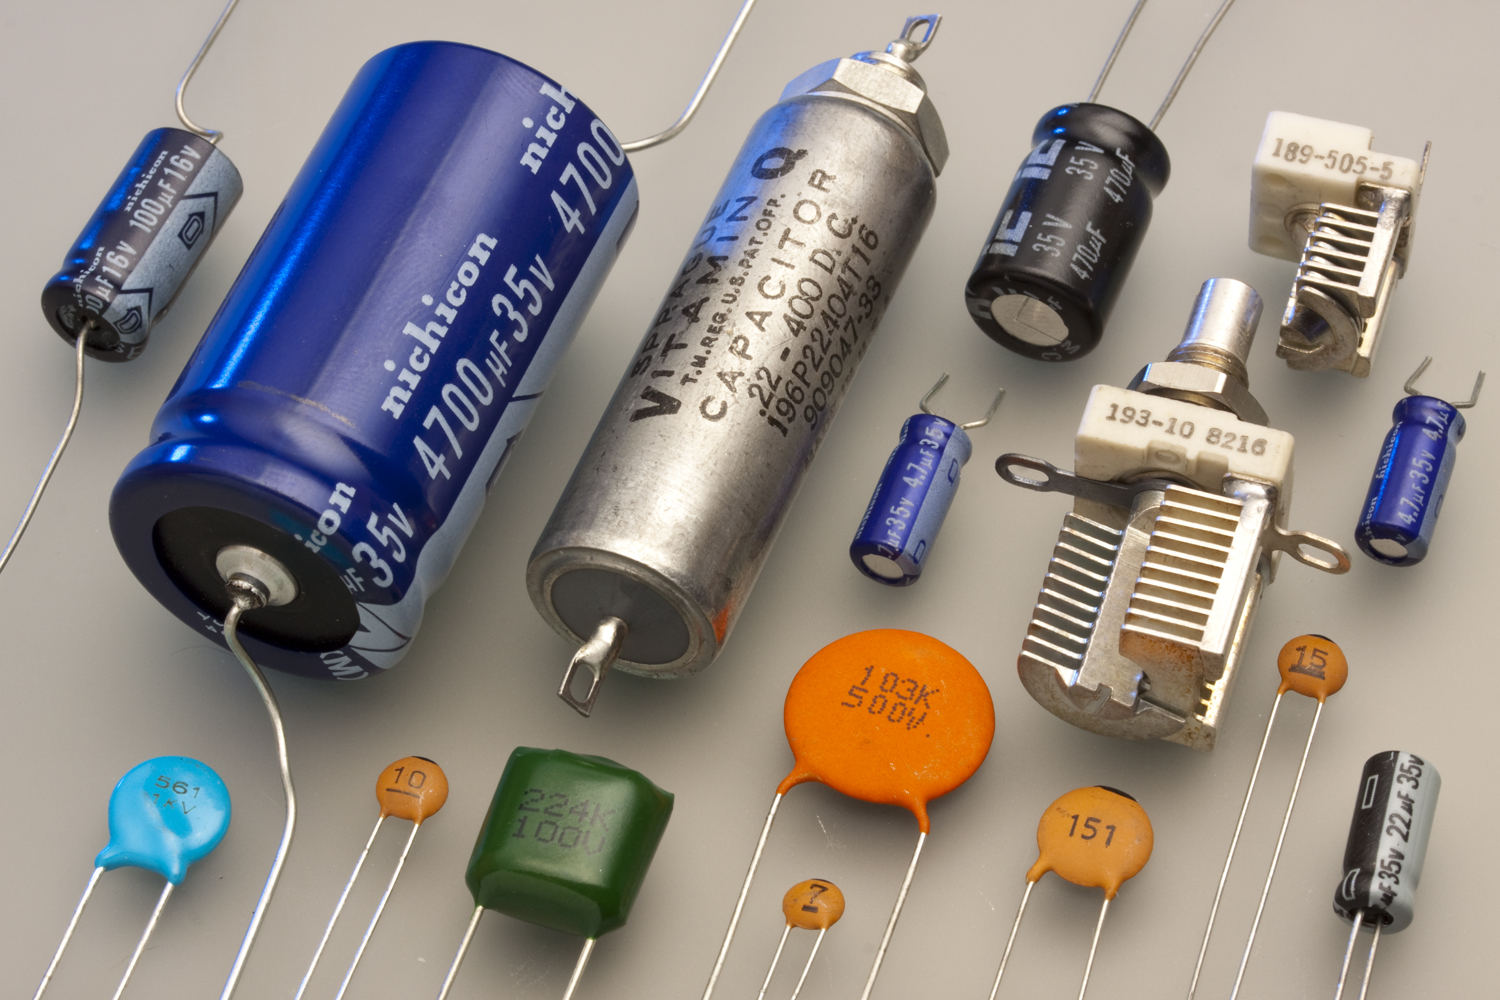
\includegraphics[width=\twowide]{capacitors}
    \caption{Components}
  \end{subfigure}
  \caption{Typical Capacitors}
  \label{fig:caps}
\end{figure}

An ideal capacitor is completely characterized by a constant
\term{capacitance}, $C$, measured in \term{farads}, symbol~\unit{F}.

The prototypical capacitor consists of two parallel conductive plates
separated by a non-conductive material or \term{dielectric}. It can be
shown that a parallel plate capacitor having two plates of area $A$,
separated by a distance $d$, filled with a dielectric of
\term{permittivity} $\epsilon$, has a capacitance given
  by\footnote{This is idealized and might more accurately be described
    as the capacitance of a section of area $A$ of an infinite
    parallel plate capacitor or at least one so large that the
    different behavior at the edges, called \term{fringing} can be
    neglected.}:
\[
C = \frac{\epsilon A}{d}\qquad\bunit{F}
\]

The relationship between current and voltage in an ideal capacitor is given by:
\begin{equation}
\label{eqn:cdvdt}
i(t) = C\deedee{v(t)}{t}
\end{equation}
Equivalently:
\[
v(t) = \frac{1}{C}\int i(t)\dee{t}
\]

The energy stored in the electric field of a capacitance of
$C~\unit{F}$, charged to a constant voltage, $V$, is given by:
\[
E = \frac{1}{2}CV^2\qquad\bunit{J}
\]

\paragraph{Transient Behavior}
\label{sec:rcstep}

Suppose a completely discharged \ruC ideal capacitor is connected at
$t=0$ (by throwing a switch) to a \ruVdc battery having an internal
resistance of \ruR as shown in Figure~\ref{fig:rcseries}.

\begin{figure}[H]
  \centering
  \begin{circuitikz}
    \draw (0,0) node[ground] {};
    \draw (0,0) to [V=$\ruVdc$] (0,2);
    \draw (0,2) to [R=$\ruR$, v=$v_\mathrm{R}$] (2,2);
    \draw (2,2) to [spst] (4,2);
    \draw (4,2) to [C=$\ruC$, v=$v_\mathrm{C}$] (4,0);
    \draw (4,0) to [short] (0,0);
  \end{circuitikz}
  \caption{A Capacitor Connected to a Battery}
  \label{fig:rcseries}
\end{figure}

By Kirchoff's Voltage Law (the sum of the voltages around a loop is zero),
\begin{equation}
\label{eqn:rckvl}
v_\mathrm{R} + v_\mathrm{C} = V_\mathrm{B}\quad \left(\ruVdc\right)
\end{equation}

There is only one possible current path, so:
\[
i_\mathrm{R} = i_\mathrm{C}
\]

By substitution, using~\eqref{eqn:vir} and~\eqref{eqn:cdvdt}:
\[
\frac{v_\mathrm{R}}{R} = C\deedee{v_\mathrm{C}}{t}
\]
or, by~\eqref{eqn:rckvl}\footnote{It's slightly more convenient to
  solve for $v_\mathrm{R}$ than $v_\mathrm{C}$}:
\[
\frac{1}{RC} v_\mathrm{R} = \deedee{t} V_\mathrm{B} - \deedee{t} v_\mathrm{R}
\]
The battery voltage is constant, so rearranging:
\[
\deedee{t} v_\mathrm{R} + \frac{1}{RC} v_\mathrm{R} = 0
\]
The solution to this well-known homogeneous ODE (subject to the
initial condition $v_\mathrm{R}(0)=V_\mathrm{B}$) is:
\[
v_\mathrm{R}(t) = V_\mathrm{B} e^{-\frac{t}{RC}}
\]
By Ohm's Law:
\[
i(t) = \frac{v_\mathrm{R}(t)}{R} = \frac{V_\mathrm{B}}{R} e^{-\frac{t}{RC}}
\]
And, by~\eqref{eqn:rckvl}:
\[
v_\mathrm{C}(t) = V_\mathrm{B}\left(1 - e^{-\frac{t}{RC}}\right)
\]
Plotting with the values for $V_\mathrm{B}$, $R$, and $C$ given above
(\ruVdc, \ruR, and \ruC, respectively) yields Figure~\ref{fig:rcstep}.

\begin{figure}[ht]
  \centering
  \includegraphics[width=\onewide]{rcstep}
  \caption{Step Response of a Series RC Circuit}
  \label{fig:rcstep}
\end{figure}

The value $RC$ is called the \term{time constant} and has units of
seconds\footnote{A farad is a second per ohm.}:
\[
\tau = RC = \ruR\times\ruC = \ruTauC
\]
$v_\mathrm{C}(t)$ can be written:
\[
v_\mathrm{C}(t) = V_\mathrm{B}\left(1 - e^{-\frac{t}{\tau}}\right)
\]


\paragraph{DC Behavior}

It should be clear from the foregoing analysis that the steady-state
DC behavior of a capacitor is to block DC current flow. In other
words, a capacitor behaves like an \emph{open circuit} to DC.


\paragraph{AC Behavior}

The capacitor's frequency-dependent AC analog of resistance is
\term{capacitive reactance}. It is inversely proportional to
capacitance and frequency and is given by:
\[
X_\mathrm{C} = \frac{1}{\omega C} = \frac{1}{2\pi f C} \qquad\bunit{\Omega}
\]

Dimensionally:
\[
X_\mathrm{C} = \frac{1}{\omega\bunit{1}{s}\cdot C~\bunit{F}} = \unit{s}\cdot\unit{1}{F} = \unit{s}\left(\unit{\Omega}{s}\right) = \unit{\Omega}
\]

In short, a fixed-value ideal capacitors's reactance is inversely
proportional to frequency. This is consistent with what we know about
the capacitor's DC behavior since, loosely speaking: at zero frequency
(DC), the reactance is infinite.

Since an ideal capacitor is a pure energy storage device, under
quasi-static conditions (AC voltage applied for a long time), any
power stored during one part of a cycle is returned during another
part of the cycle.

If we were to apply the nominal domestic service voltage to our \ruC
capacitor, we would see the voltage and current shown in
Figure~\ref{fig:capac}. Note that the current scale is
\emph{milliamps}.

\begin{figure}
  \centering
  \includegraphics[width=\onewide]{capac}
  \caption{Current Leads Voltage in a Capacitor}
  \label{fig:capac}
\end{figure}

The RMS current in Figure~\ref{fig:capac} is
$\approx\ruImC$. In time, the current leads voltage by 90\deg.


\paragraph{Colloquialisms}

A real capacitor is sometimes called a \term{cap}.


\subsubsection{Inductor}

\begin{figure}[H]
  \centering
  \begin{subfigure}[b]{\twowide}
    \centering
    \begin{circuitikz}
      \draw (0,0) to [L=$1~\unit{mH}$] (2,0);
    \end{circuitikz}
    \caption{Symbol}
  \end{subfigure}
  \begin{subfigure}[b]{\twowide}
    \centering
    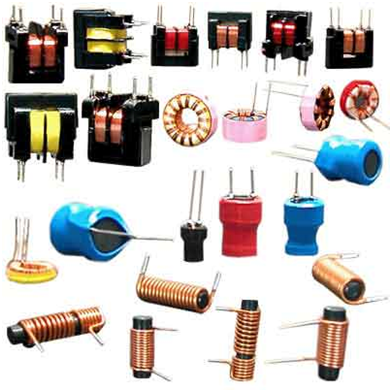
\includegraphics[width=\twowide]{inductors}
    \caption{Components}
  \end{subfigure}
  \caption{Typical Inductors}
  \label{fig:coils}
\end{figure}

An ideal inductor is completely characterized by a constant
\term{inductance}, $L$, measured in \term{henries}, symbol~\unit{H}.

The prototypical inductor consists of a helical coil of perfectly
conductive wire wound on a non-conductive cylindrical \term{core}.

It can be shown that a helical coil of length $l$ and cross-sectional
area $A$ with $n$ turns, surrounded and filled by a medium of
\term{magnetic permeability} $\mu$, has an inductance given by:
\[
L = \frac{\mu n^2 A}{l}\qquad\bunit{H}
\]

The relationship between current and voltage in an ideal inductor is given by:
\begin{equation}
\label{eqn:ldidt}
v(t) = L\deedee{i(t)}{t}
\end{equation}

Or, equivalently:
\[
i(t) = \frac{1}{L}\int v(t)\dee{t}
\]

The energy stored in the magnetic field of an inductance of
$L~\unit{H}$ carrying a constant current, $I$, is given by:
\[
E = \frac{1}{2} L I^2\qquad\bunit{J}
\]


\paragraph{Transient Behavior}

Suppose a completely discharged \ruL ideal inductor is connected at
$t=0$ (by throwing a switch) to a \ruVdc battery having an internal
resistance of \ruR as shown in Figure~\ref{fig:rlseries}.

\begin{figure}[H]
  \centering
  \begin{circuitikz}
    \draw (0,0) node[ground] {};
    \draw (0,0) to [V=$\ruVdc$] (0,2);
    \draw (0,2) to [R=$\ruR$, v=$v_\mathrm{R}$] (2,2);
    \draw (2,2) to [spst] (4,2);
    \draw (4,2) to [L=$\ruL$, v=$v_\mathrm{L}$] (4,0);
    \draw (4,0) to [short] (0,0);
  \end{circuitikz}
  \caption{An Inductor Connected to a Battery}
  \label{fig:rlseries}
\end{figure}

Following \emph{exactly} the same procedure as for the analagous
capacitor circuit in \S\ref{sec:rcstep}, above, we find that:
\[
i(t) = \frac{V_\mathrm{B}}{R}\left(1-e^{-\frac{R}{L}t}\right)
\]

\[
v_\mathrm{R}(t) = V_\mathrm{B}\left(1-e^{-\frac{R}{L}t}\right)
\]

\[
v_\mathrm{L}(t) = V_\mathrm{B}e^{-\frac{R}{L}t}
\]

Plotting with the values for $V_\mathrm{B}$, $R$, and $L$ given above
(\ruVdc, \ruR, and \ruL, respectively) yields Figure~\ref{fig:rlstep}.

\begin{figure}[ht]
  \centering
  \includegraphics[width=\onewide]{rlstep}
  \caption{Step Response of a Series RL Circuit}
  \label{fig:rlstep}
\end{figure}

In this case, the time constant is\footnote{A henry is an ohm-second.}:
\[
\tau = \frac{L}{R} = \frac{\ruL}{\ruR} = \ruTauL
\]
$v_\mathrm{L}(t)$ can be written:
\[
v_\mathrm{L}(t) = V_\mathrm{B}e^{-\frac{t}{\tau}}
\]


\paragraph{DC Behavior}

It should be clear from the foregoing analysis that the steady-state
DC behavior of an inductor is to conduct current. In other words, an
inductor behaves like a \emph{short circuit} to DC.


\paragraph{AC Behavior}

The inductor's frequency-dependent AC analog of resistance is
\term{inductive reactance}. It is directly proportional to inductance
and frequency and is given by:
\[
X_\mathrm{L} = \omega L = 2\pi f L\qquad\bunit{\Omega}
\]

Dimensionally:
\[
X_\mathrm{L} = \omega\bunit{1}{s}\cdot L~\bunit{H} = \unit{H}{s} = \left(\unit{\Omega\cdot s}\right)\cdot\unit{1}{s} = \unit{\Omega}
\]

In short, a fixed-value ideal inductor's reactance increases linearly
with frequency. This is consistent with what we already know about the
inductor's DC behavior since, loosely speaking: at zero frequency
(DC), the reactance is zero (a short circuit).

Since an ideal inductor is a pure energy storage device, under
quasi-static conditions (AC voltage applied for a long time), any
power stored during one part of a cycle is returned during another
part of the cycle.

If we were to apply the nominal domestic mains service voltage to our
\ruL inductor, we would see the voltage and current shown in
Figure~\ref{fig:indac}. Note that the current scale is
\emph{amperes}\footnote{And to handle the $\approx\ruIpL$ peak
  current, this would have to be one hefty inductor!}.

\begin{figure}
  \centering
  \includegraphics[width=\onewide]{indac}
  \caption{Voltage Leads Current in an Inductor}
  \label{fig:indac}
\end{figure}

The RMS current in Figure~\ref{fig:indac} is $\approx\ruImL$. In time,
voltage leads current by 90\deg in an inductor.

\paragraph{Colloquialisms}

A real inductor is often colloquially called a \term{coil}. 

A \term{choke} is an inductor used to suppress high-frequency
currents.


\subsubsection{Complex Impedance}

\tikz \draw (0,0) to [generic=$1+\mathrm{j}5~\unit{\Omega}$] (2,0);

A \term{complex impedance}, $Z$ has a resistive component, $R$, and a
reactive component, $X$:

\[
Z = R + \mathrm{j}X
\]

The reactive component $X$ may be a capacitive reactance:
\[
Z = R - \mathrm{j}X_\mathrm{C} = R - \mathrm{j}\cdot\frac{1}{\omega C}
\]
or an inductive reactance:
\[
Z = R + \mathrm{j}X_\mathrm{L} = R + \mathrm{j}\cdot\omega L
\]

If the reactive component of impedance, $\Im(Z)$, is:
\begin{itemize}
  \item \emph{zero}, $\Im(Z)=0$, the impedance is termed \term{purely resistive}.
  \item strictly \emph{positive}, $\Im(Z)>0$, the impedance is termed \term{inductive}.
  \item strictly \emph{negative}, $\Im(Z)<0$, the impedance is termed \term{capacitive}.
\end{itemize}

Suppose we consider a series RL circuit --- similar to that considered
before --- consisting of a \ruR resistor and a \ruL inductor in series
as shown in Figure~\ref{fig:indload}.

\begin{figure}[H]
  \centering
  \begin{circuitikz}
    \draw (0,0) node[ground] {};
    \draw (0,0) to [sV=$v$] (0,4);
    \draw (0,4) to [short, i=$i$] (3,4);
    \draw (3,4) to [R=$\ruR$] (3,2);
    \draw (3,2) to [L=$\ruL$] (3,0);
    \draw (3,0) to [short] (0,0);
  \end{circuitikz}
  \caption{An Inductive Load Connected to an AC Voltage Source}
  \label{fig:indload}
\end{figure}

%% ASSUMPTION: \rnL is in mH
Its impedance at \ruF is:
\[
Z = \rnR + \mathrm{j} \cdot \rnVm\pi \cdot \rnL\times 10^{-3} \approx \ruZ
\]

If we applied the nominal domestic mains service voltage --- \ruVm at
\ruF --- to this impedance, the current would be as depicted in
Figure~\ref{fig:srlac}.

\begin{figure}
  \centering
  \includegraphics[width=\onewide]{srlac}
  \caption{Voltage and Current in an Inductive Impedance}
  \label{fig:srlac}
\end{figure}

We can see that voltage is still leading current, as we would expect
from the inductance, but by a bit less than 45\deg, not 90\deg.

The exact relationship can be computed surprisingly easily: we just
apply Ohm's Law using phasors:
\begin{equation}
\label{eqn:acohms}
i = \frac{\abs{V_\mathrm{p}}\angle0}{Z} = \frac{(\rnVm\sqrt{2})\angle0}{\rnZ} \approx \frac{\rnVp\angle0}{\rnModZ\angle\rnArgZ\deg} = \rnModI\angle{\rnArgI}
\end{equation}
This tells us that the current peaks at \ruModI and lags the voltage by
\ruAbsArgI. Equivalently, we can say that \emph{voltage leads current}
by \ruAbsArgI.


\subsubsection{Transformer}



\section{Single-Phase Power}

Because of the phase relationship between current and voltage, AC
\emph{power} is not as simple as the DC case. Only in the case of a
purely resistive load --- one with no reactive component, capacitive
or inductive --- is RMS power, the product of RMS voltage and RMS
current, meaningful.

\begin{figure}[H]
  \centering
  \begin{circuitikz}
    \draw (0,0) node[ground] {};
    \draw (0,0) to [sV=$\ruVm$] (0,2);
    \draw (0,2) to [short] (2,2);
    \draw (2,2) to [generic=$Z$] (2,0);
    \draw (2,0) to [short] (0,0);
  \end{circuitikz}
  \caption{A Generic Load Connected to an AC Source}
  \label{fig:acload}
\end{figure}

Provided that we deal in complex numbers, however, power obeys a
simple and somewhat familiar equation, but note the complex conjugate
of the current:

\[
S = \bar{i} \times v
\]

Where $S$ is a complex number:

\[
S = P+\mathrm{j}Q
\]

Here $S$ is the \term{apparent power} in \term{volt-amperes}
(\unit{VA}), $P$ is the \term{real power} in watts (\unit{W}), and $Q$
is the \term{reactive power} in \term{reactive
  volt-amperes}\footnote{Or, if you prefer alignment with the
  abbreviation over grammar, ``volt-amperes, reactive'' or
  ``volt-amperes (reactive)''.} (\unit{VAr}).

\begin{figure}[ht]
  \centering
  \includegraphics[width=\onewide]{acpower}
  \caption{AC Power: $S=P+\mathrm{j}Q$}
  \label{fig:acpower}
\end{figure}


If $Z$ in Figure~\ref{fig:acload} is the RL series arrangement of
Figure~\ref{fig:indload}, the voltage, current, and power phasors are
as shown in Figure~\ref{fig:pwrphasor}. Well, almost: the lengths of
the phasors in Figure~\ref{fig:pwrphasor} are $\log_{10}$ of their
normal linear values so we can ``see everything'', and we're more
interested in the phase relationships at this point.

\begin{figure}[ht]
  \centering
  \includegraphics[width=\onewide]{pwrphasor}
  \caption{Voltage, Current, and Power Phasors}
  \label{fig:pwrphasor}
\end{figure}


\subsubsection{Power Factor}

The \term{power factor} is the ratio of real to apparent power:
\[
\lambda = \frac{\abs{P}}{\abs{S}} = \cos\phi \qquad \in [0,1]
\]

A \term{purely resistive} load has a power factor of 1. A \term{purely
  inductive} load \emph{or} a \term{purely capacitive} load has a
power factor of 0, since there is no real power in either case: $P=0$.

A capacitive load is differentiated from an inductive load by
appending ``lagging'' in the case of an inductive load or ``leading''
in the case of an inductive load. In the context of power factor,
voltage is \emph{always} considered the reference. So if current lags
voltage, the load is inductive, and if current leads voltage, the load
is capacitive.

Looking at Figure~\ref{fig:pwrphasor} again, the current phasor (red)
appears clockwise of the voltage phasor (blue). The angle? We
calculated that in Equation~\ref{eqn:acohms}: \ruArgZ. The angle
subtended by the apparent power, $S$, to the real axis is the same, so
the power factor in this case is \rnPF.

Although the usual definition of power factor doesn't admit the
possibility of negative power factors, they have been used
historically with differing conventions and there is an argument that
``negative power'' is a more useful concept today, when domestic
rooftop solar and other small-scale generators have turned what would
traditionally have been loads into ``sometimes loads, sometimes
generators''.

Note that, in general, although we usually shorten ``ampere'' to
``amp'' colloquially, this is done less often with units that
``compound'' the ampere with other units, such as
ampere-second\footnote{aka coulomb, $1\unit{C}=1\unit{A\cdot s}$},
volt-ampere (\unit{VA}), or ampere-hour (\unit{Ah}).


\subsection{Lagging and Leading}

The issue of what is considered lagging and leading causes
considerable confusion.

Clearly, ``$X$ lags $Y$'' is the same as saying ``$Y$ leads
$X$''. Neither of these are meaningful if $X$ and $Y$ differ in
frequency, but their amplitudes are irrelevant: lagging and leading
are purely about time.

There are four sources of confusion:
\begin{itemize}
  \item Current and voltage vs. time plots ``look'' backwards (to many people at least);
  \item The standard mnemonic mixes \emph{current} and \emph{voltage} as the reference
  \item Power factor consistently uses \emph{voltage} as the reference
  \item A lagging (or leading) power factor phasor points different
    directions depending on what is plotted
\end{itemize}

\subsubsection{Backwards Plots}

If $X$ leads $Y$, this means that $X$'s sinusoid appears shifted
\emph{to the left} with respect to $Y$'s. $X$ is leading \emph{in
  time}, so its ``events'' (zero-crossings, peaks, troughs) happen
\emph{sooner} (to the left).

This can be confusing, because it's the opposite way around from what
one might intuitively and reasonably expect looking at a graph: that
``leading'' means ``looks shifted to the right'', which is the exact
opposite of what it really means: if $X$ \emph{leads} $Y$, then $X$
appears shifted to the \emph{left} --- sooner in time --- with respect
to $Y$.

Similarly, if $X$ \emph{lags} $Y$, then $X$ appears shifted \emph{to
  the right} --- later in time --- with respect to $Y$.

\subsubsection{Mnemonic Mixes Reference Signals}

The (strained) mnemonic used to remember the ``what leads
what'' in inductors and capacitors is:

\begin{quote}
\centering
ELI the ICE man
\end{quote}

Where ``E'' stands for voltage, ``I'' stands for current, ``L''
stands for inductance, and ``C'' stands for capacitance,

\begin{itemize}
  \item {\bf ELI} means ``voltage leads current in an inductor''\footnote{The ``L'' for inductor is ``in'' the middle, gettit? Yes, I think it's pretty stupid too.}
  \item {\bf ICE} means ``current leads voltage in a capacitor''
\end{itemize}

The problem here is that the relationship, ``leads'', is implied. It's
easy to misremember it as ``lags'' and get everything backwards.


\subsubsection{Power Factor Uses Voltage as Reference}

Mercifully and sensibly, power factor consistently uses voltage as the reference:

\begin{itemize}
  \item If PF is ``lagging'', then current \emph{lags} voltage
    (inductive), and the current phasor points ``down'', somewhere in
    the lower right quadrant.
  \item If PF is ``leading'', then current \emph{leads} voltage (capacitive), and the current phasor points ``up'', somewhwere in the upper right quadrant.
\end{itemize}


\subsubsection{Complex Values Point Different Directions}

The current phasor for a lagging power factor points down, but the
power phasor for a lagging power factor points up. An inductive
impedance, though not a phasor, can be (and often is) plotted on the
same Argand diagram and points up.

The current phasor for a leading power factor points up, but the power
phasor for a leading power factor points down. A capacitive impedance
points down.

Though it makes sense when you work through it, it can be confusing
keeping all of this ``straight'' in your head. The two key things to
remember are: 
\begin{itemize}
  \item that the definition of apparent power uses \emph{the complex
  conjugate} of the current, so the apparent power phasor will
    \emph{always} lie on the mirror-image of the current phasor.
  \item that the current is the voltage \emph{divided by} the complex
    impedance, so the current phasor will \emph{always} lie on the
    mirror-image of the complex impedance plotted on the same Argand
    diagram.
\end{itemize}

Given these two facts, it should be no surprise that the complex
impedance points the same way as the apparent power phasor, as it lies
on the mirror-image of a mirror-image.

\section{Essential Principles}

\subsection{Kirchoff's Voltage Law}

The sum of the potential differences around a closed loop is zero
(just conservation of potential energy).

\subsection{Kirchoff's Current Law}

The sum of the currents into a node is zero (just conservation of
mass: where else could electrons go?)

\subsection{Th\'evenin's Theorem}

Any linear one-port circuit is equivalent to a voltage source in
series with an impedance.

\subsection{Norton's Theorem}

Any linear one-port network is equivalent to a \emph{current} source
in \term{parallel} with an impedance.

\subsection{Duality of Th\'evenin's and Norton's Theorems}

Th\'evenin's Theorem is the dual of Norton's theorem (next): any
one-port network that has a Norton equivalent circuit has a
Th\'evenin's equivalent circuit and {\it vice versa}.

The Norton equivalent and Th\'evenin equivalent impedances for any
network are the same.

In practice, Th\'evenin equivalent circuits are more common than
Norton equivalent circuits.


\subsection{Maximum Power Transfer (MPT) Theorem}

Any Th\'evenin equivalent one-port network transfers maximum power to
a load when the load's impedance is the complex conjugate of the
network's Th\`evenin equivalent series impedance.

By duality, this applies equally to a Norton equivalent circuit.


\section{Semiconductors}

\subsection{Diode}

Semiconductor diodes can be, broadly speaking, divided into
\term{small signal} and \term{power} types. Small signal diodes come
in a bewildering number of varieties\footnote{Even leaving aside
  light-emitting diodes, laser diodes, photodiodes, etc.} (microwave
resonant tunnel diodes, anyone?). For power purposes, however, there
are relatively few significant variations.

There are a few different levels of ``ideality''. To a first
approximation, an ideal diode behaves much like a flap valve, letting
current flow one way, but not the other, and has zero resistance. At
the next level, the diode's I-V characteristic follows the Shockley
equation:
\[
I = I_\mathrm{S}\left(e^{\left(\frac{V}{V_\mathrm{T}}\right)}-1\right)
\]

\ldots where $I$ and $V$ are the diode current and voltage,
respectively, $I_\mathrm{S}$ is the \term{reverse saturation current},
which could be anywhere between about 1~\unit{nA} and a few~\unit{\mu
  A}, but usually between a few and a few tens of \unit{nA}, \and
$V_\mathrm{T}$ is the \term{thermal voltage}:
\[
V_\mathrm{T} = \frac{kT}{q} \approx 25.85\,~\unit{mV}\qquad \text{(at 300\,~\unit{K})}
\]

Figure~\ref{fig:shockley} plots the Shockley equation for a reverse
saturation current of 20~\unit{nA}. Note that this diode has a forward
current of \term{over a billion amps} at one volt: it is effectively a
short circuit at any forward voltage more than a few hundred
millivolts.

\begin{figure}[ht]
  \centering
  \includegraphics[width=\onenarrow]{shockley}
  \caption{Ideal Diode with $I_\mathrm{S}=20\,\unit{nA}$}
  \label{fig:shockley}
\end{figure}


Figure~\ref{fig:ivdiode} shows a cartoon representation of the
current-voltage behavior of a typical non-ideal semiconductor
diode. {\bf Note that this is not to scale: }the reverse current is
typically minuscule (sub-\unit{\mu A}) compared to the forward current
(\unit{mA} to \unit{kA} depending on application), at least until
breakdown, and the reverse breakdown voltage is typically orders of
magnitude larger (tens to thousands of volts) than the forward voltage
drop (hundreds of~\unit{mV}).

\begin{figure}[ht]
  \centering
  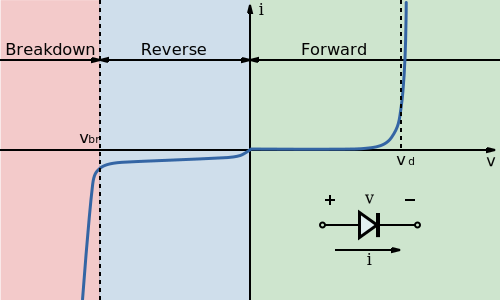
\includegraphics[width=\onenarrow]{ivdiode}
  \caption{Generic Diode I-V Characteristic Cartoon}
  \label{fig:ivdiode}
\end{figure}


\subsubsection{Rectifier}

Rectifier diodes are power diodes available in current ratings from
perhaps 500~\unit{mA} to 10~\unit{kA}.

The principal ratings are the maximum forward current, peak inverse
voltage (PIV), forward voltage drop. A typical small ``vanilla''
silicon rectifier can carry a few amps, has a PIV ratings between
maybe 100 and 1,000 volts, drops about 0.7~\unit{V}, and can switch
fast enough for mains service.

A \term{Schottky diode} has much lower forward voltage drop, about
0.2~\unit{V}, and higher switching speed, suitable for high-speed
switching circuits, but at the expense of much lower PIV rating.

\paragraph{Zener Diode}

A \term{Zener diode} is a diode engineered so that the reverse
breakdown voltage\footnote{Colloquially referred to as ``the knee''.}
is consistent, non-destructive, and nearly constant with
current. Zener diodes are typically used as voltage references.

Many diodes colloquially called ``Zener diodes'' are technically
\term{avalanche diodes} as there are two subtly different reverse
breakdown effects: the Zener effect and the avalanche effect.


\subsection{Bipolar Junction Transistor (BJT)}



\subsection{Field Effect Transistor (FET)}


\section{Three-Phase Power}

Three-wire system. Optional fourth (neutral) wire.

Three \term{phases} (sinusoidal AC voltages), each $\frac{2\pi}{3}$ or
120\deg out-of-phase with the other two as shown in
Figure~\ref{fig:threephase}.

\begin{figure}[ht]
  \centering
  \includegraphics[width=\onewide]{threephase}
  \caption{120/208\,\unit{V} 3-phase Power}
  \label{fig:threephase}
\end{figure}

A 3-phase system can be described either by the
\term{phase-to-neutral} or \term{phase-to-phase} voltages:
\[
V\mathrm{LL} = \sqrt{3}V\mathrm{LN}
\]
$V\mathrm{LL}$ (live-to-live) is used rather than $V_\mathrm{PP}$ to
avoid confusion with peak-to-peak voltage.
 
Often, 3-phase service/supply is redundantly described by the two
values separated by a slash, e.g. 120/208, 240/415, or 277/480. Note
that both voltages in all cases are RMS values.

\begin{figure}[ht]
  \centering
  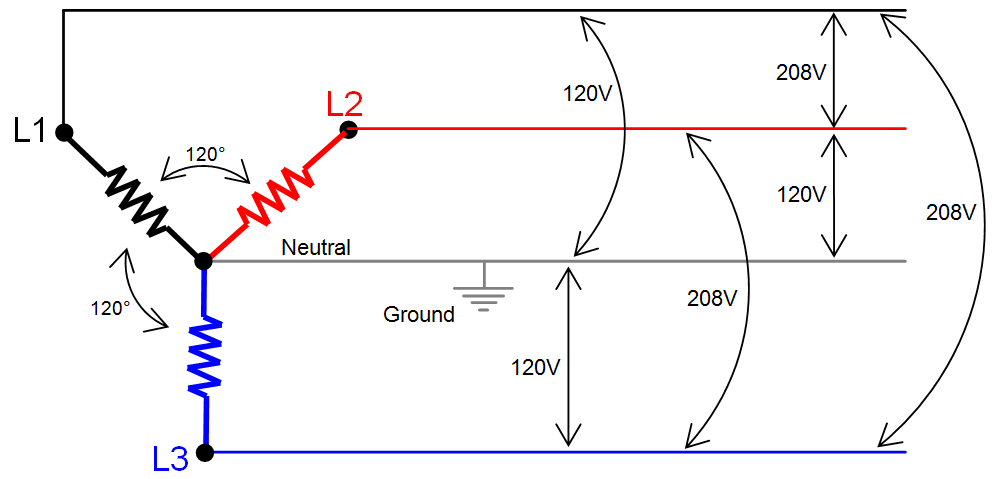
\includegraphics[width=\onewide]{wyevoltages}
  \caption{120/208\,\unit{V} Wye-Connected Power}
  \label{fig:wyevoltages}
\end{figure}

\subsection{Delta and Wye Connections}

\subsection{Why Three?}

Triple power for 50\% extra copper (delta, no neutral, at HV).

Very nice rectification properties, as shown in
Figure~\ref{fig:nicerect}. Ripple frequency is six times supply
frequency and amplitude is about 13\% of phase-to-neutral amplitude.

\begin{figure}[ht]
  \centering
  \includegraphics[width=\onewide]{nicerect}
  \caption{Rectified 3-Phase}
  \label{fig:nicerect}
\end{figure}



Go to $n$-phase, get $\frac{n-3}{3}$ extra power for $\frac{n-31}{3}$
extra copper --- no economic advantage. 

Even numbers of phases don't have nice rectification properties.



\subsection{Per-Unit System}


\section{Rotating Electric Machines}

There is a saying in power engineering that ``all machines are
AC machines''.

DC machines are only DC via commutation.

Mechanical:
\begin{itemize}
  \item \term{rotor} --- rotating part
  \item \term{stator} --- fixed part
\end{itemize}

Electromagnetic:
\begin{itemize}
  \item \term{armature winding} --- power supply/take-off; all machines have at least one armature winding. 
  \item \term{field winding} --- provides magnetic field; permanent-magnet machines have no field winding(s).
\end{itemize}


\subsection{Motor}

An \emph{electric motor} is a device that converts electrical power
into mechanical rotational power.

Tend to think in terms of simple unipolar permanent magnet motor.

A motor with a constant magnetic field, either permanent magnet or
DC-excited field winding(s), has a motor constant $K_v$ in
\unit{RPM}{V}.


\subsection{Generator}

A \emph{generator} is a device that converts mechanical rotational
power into electrical power.

The mechanical-to-electrical conversion efficiency of a large
generator typically exceeds 98\%.



\section{The Grid}

\subsection{Transmission}

\subsubsection{High-Voltage DC}

Long-distance transmission, e.g. Pacific DC Intertie (3\,\unit{GW}, 3\,\unit{MV} at 1\,\unit{kA}).

Advantages:
\begin{itemize}
  \item Two-wire. 
  \item Relatively low current. 
  \item Uses all the copper (no skin effect).
  \item Electronic phase matching/regulation.
\end{itemize}

\begin{itemize}
  \item Corona losses.
  \item Expensive rectifiers and inverters.
\end{itemize}

\subsection{Distribution}


\subsection{Regulation}





\section{Rotational Kinetic Energy}

The blade assembly of a wind turbine can be viewed as a device that
converts the translational kinetic energy of the wind to rotational
kinetic energy (RKE).

Rotational kinetic energy (in joules) of the ``turning parts'' ---
including the blade, hub, shaft, etc. --- is given by\footnote{Note
  the similarity to the expression for \emph{translational} KE:
  $\frac{1}{2}mv^2$.}:

\begin{equation}
\label{eqn:rke}
E_{rot} = \frac{1}{2}I\omega^2
\end{equation}

Where $I$ is the \term{moment of inertia} (in \unit{kg\cdot m^2}) of
the blade assembly around the hub axis and $\omega$ is its
\emph{angular velocity} (in \unit{rad}{s}). 

The rotational \emph{power} (in watts) is, via Newton's Laws, the time
derivative of the RKE:

\begin{equation}
\label{eqn:rpow}
P_{rot} = \frac{I}{2}\deedee{\omega^2}{t} = I\omega
\end{equation}


\clearpage
\appendix

\section{Rotational Mechanics}

Table~\ref{tbl:rotquant} summarizes the rotational analogues of the
more familiar translational quantities.

\begin{table}[H]
  \centering
  \begin{tabular}{lccccl} \toprule
    \multicolumn{3}{c}{Linear Mechanics} & \multicolumn{3}{c}{Rotational Mechanics} \\ \cmidrule(r){1-3} \cmidrule(l){4-6}
  Name           & Unit                & Symbol                & Symbol                        & Unit                  & Name                        \\ \midrule
  Displacement   & \unit{m}            & $x$                   & $\theta$                      & \unit{rad}            & Angular Displacement        \\
  Mass           & \unit{kg}           & $m$                   & $I$                           & \unit{kg\cdot m^2}    & Moment of inertia           \\
  Velocity       & \unit{m}{s}         & $v = \deedee{x}{t}$   & $\omega = \deedee{\theta}{t}$ & \unit{rad}{s}         & Angular Velocity            \\
  Momentum       & \unit{kg\cdot m}{s} & $p = mv$              & $L = I\omega$                 & \unit{kg\cdot m^2}{s} & Angular Momentum            \\
  Acceleration   & \unit{m}{s^2}       & $a = \deedee{v}{t}$   & $\alpha = \deedee{\omega}{t}$ & \unit{rad}{s^2}       & Angular Acceleration        \\
  Force          & \unit{N}            & $F = ma$              & $T = I\alpha$                 & \unit{N\cdot m}       & Torque                      \\
  Work           & \unit{J}            & $W = F\dee{x}$        & $W = T \dee{\theta}$          & \unit{J}              & (Rotational) Work           \\
  Kinetic Energy & \unit{J}            & $E = \frac{1}{2}mv^2$ & $E = \frac{1}{2}I\omega^2$    & \unit{J}              & (Rotational) Kinetic Energy \\
  Power          & \unit{W}            & $P = Fv$              & $P = T\omega$                 & \unit{W}              & (Rotational) Power          \\ \bottomrule
  \end{tabular}
  \caption{Linear Quantities and Their Rotational Analogs}
  \label{tbl:rotquant}
\end{table}

By way of example, \term{moment of inertia} is the analog of {mass} in
translational mechanics. In the same way as the mass, $m$, (in
\unit{kg}) can be viewed as the property of an object that determines
the force, $F$, (in \unit{N}) required for a particular \emph{linear}
acceleration, $a$, (in \unit{m}{s^2}) --- $F=ma \implies
m=\frac{F}{a}$ --- moment of inertia, I, determines the \emph{torque},
$T$, (in \unit{N\cdot m}) required for a particular \emph{angular}
acceleration (in \unit{rad}{s^2}): $\tau=I\alpha \implies
I=\frac{\tau}{\alpha}$.


\end{document}
